%%
%% Author: thompson
%% 01.11.17
%%

% Preamble
\documentclass[11pt]{article}

% Packages
\usepackage{a4wide}
\usepackage[utf8]{inputenc}
\usepackage[ngerman]{babel}

\usepackage{enumerate}
\usepackage{scrextend}
\usepackage{graphicx}

% Document
\begin{document}
    \section{Protokolle der Anwendungsschicht}
    Konsultieren Sie sogenannte RFCs der IETF (erklären Sie die Bedeutung dieser
    Abkürzungen) um folgende Fragestellungen zu beantworten:

    \begin{enumerate}[\thesection .1]
    \item Beschreiben Sie die folgenden Protokolle hinsichtlich ihrer Eigenschaften und
wesentlichen Unterschiede: HTTP/0.9, HTTP/1.0, HTTP/1.1, HTTP/2.0.

    \begin{enumerate}[$\diamond$]
        \item \textbf{HTTP/0.9} :: Erstellt 1991.\\ Es ist ein Subset des vollen HTTP-Protokolls, wie wir es heute kennen.\\
        Merkmale:
        \begin{addmargin}[1em]{1em}
            \begin{enumerate}
                \item Kein Austausch von Klientenprofil.
                \item Einfachheit Request/Response-Model
                \item Keine Sessions oder States
                \item Weitverbreitete Nutzung: Request of Data through Browser
                \item Nutzt telnet-Protokolstil via TCP-IP\\
            \end{enumerate}
        \end{addmargin}

        \underline{Beispiel: Verbindungsaufbau}\\
        Der Klient erstellt eine TCP-IP Verbindung zu einem Host via Domänname oder IP und Port-Nummer.
        Wird kein Port definiert, so wird der default-Wert 80 gesetzt.
        Der Server akzeptiert die Verbinung und Datentransfer kann stattfinden.
    \begin{addmargin}[1em]{1em}
        \emph{telnet mailsrv.aau.at 25} ... verbindung zum Mailserver der AAU auf Port 25\\
    \end{addmargin}

        \underline{Beispiel: Request \& Response}\\
        Ein HTTP-Request wird an einen Server gestellt.
        \begin{addmargin}[1em]{1em}
            \emph{"GET http://www.uni-klu.ac.at:80/myapp/index.html"}
        \end{addmargin}
        Der Server überprüft diese Anfrage.
        \begin{addmargin}[1em]{1em}
            Gibt es dieses Dokument?\\
            Darf der User darauf zugreifen?\\
            Ist es ein dynamisch generiertes Dokument?\\
            Ist das GET-Format richtig? ... u.s.w.
        \end{addmargin}
        Der Server sendet anschließend eine Nachricht zurück zum Anfragensteller.\\
        \footnote[1 Vgl.: HTTP-Statuscodes]{Siehe https://de.wikipedia.org/wiki/HTTP-Statuscode}
        \begin{addmargin}[1em]{1em}
            Information - 100++: Continue, Switching Protocols, Processing\\
            Erfolgreich - 200++: OK, Accepted, Non-Authoritative Information,...\\
            Umleitungen - 300++: Moved permanently, See other, Use \footnote[2 Proxy]{A proxy is a
            forwarding agent, receiving requests for a URI in its absolute form,
            rewriting all or parts of the message, and forwarding the reformatted
            request toward the server identified by the URI.}, ...\\
            Client-Fehler - 400++: Bad Request, Unauthorized, Forbidden, Not Found, ...\\
            Server-Fehler - 500++: Internal Server Error, Bad \footnote[3 Gateway]{A gateway is a
            receiving agent, acting as a layer above some other server(s) and, if
            necessary, translating the requests to the underlying server's
            protocol.}, Service N/A,...
        \end{addmargin}
        Der Browser des Anfragenstellers erhält das Dokument und rendert gemäß .css/.php/... .
        Bei vollständiger Übertragung des abgerufenen Protokolls unterbricht der Server die Verbindung zum Klienten.\\

        \item \textbf{HTTP/1.0} :: Erweitert um 1994
        Spezifiziert im RFC 1945. Dies erweitert das HTTP/0.9 Protokoll um weitere TCP-IP Verbindungen für multiplen Datentransfer mittels desselben Requests.
        Dadurch werden neben Texten des eigentlichen Dokuments eingebettete Bilder, anhand deren Domäne, geladen.\\
        Eine Website welche 5 Bilder beinhaltet besitzt somit 6 Separate TCP-Verbindungen:
        \begin{addmargin}[1em]{1em}
            - 1. Verbindung: Text\\
            - 2. Verbindung: Bild 1\\
            - 3. Verbindung: Bild 2\\
            - ...\\
            - 6. Verbindung: Bild 5
        \end{addmargin}
        Es unterstützt das Caching via Header durch If-Modified-Since.\\

        \item \textbf{HTTP/1.1} :: Implementiert 1996
        Spezifiziert im RFC 2616
        Im Rahmen von HTTP/1.1 wurde das Protokoll um mehrere Funktionen erweitert:
        \begin{addmargin}[1em]{1em}
            - Support persistenter Verbindungen :: Multiple Requests über eine spezifische Leitung\\
            - Support für Packettransfer sowie Kompression \& Dekompression\\
            - Virtual Hosting :: Webserver mit 1 IP kann mehrere Domännamen besitzen\\
            - Verbesserung von Byte Transfers: Wiederaufnahme unterbrochener Vermittlungen\\
            - Sprachensupport\\
            - Funktionserweiterungen 'OPTIONS', 'PUT', 'DELETE',...
        \end{addmargin}
        Für 1.1 braucht es einen spezifizierten Header für den Host, welcher mitunter die Verbindungsart (normal, persistent) mitbestimmt.
        Dadurch kann es zu Kompatibilitätsproblemen kommen. Durch HTTP-Pipelining können mehrere Requests \& Responses innerhalb derselben Verbindung stattfinden.\\
        Im Vergleich zu 1.0, brauchte man quasi per Element eine eigene Verbindung, hier jedoch nicht. Der Transfer aller Elemente geschieht durch diesselbe TCP-Verbindung, was auch
        der Zeitkomplexität zugute kommt.
        Man kann im Rahmen des HTTP/1.1 auch Daten dem Server übertragen, mittels PUT und DELETE.\\

        \item \textbf{HTTP/2.0} :: Erstmals 2015
        Spezifiziert von der IETF als Nachfolger von HTTP/11 und definiert in RFC 7540 und 7541.
        Primär auf Optimierungen bezogen, gelten folgende Änderungen:
        \begin{addmargin}[1em]{1em}
            - Übertragungsbeschleunigung mittels Zusammenfassen mehrerer Requests :: via Multiplex\\
            - Erweiterungen der Datenkompression :: HPACK-Algorithmus, Kompression beinhaltet Kopfdaten\\
            - Binär kodierte Übertragung von Inhalten
            - Server-initiierte Datenübertragung :: Push-Verfahren\\
        \end{addmargin}

        \textbf{HTTP-Requestmethoden}:
        \begin{addmargin}[1em]{1em}
            GET: Parameterübergabe in der URL. Gekennzeichnet durch das '?'
            \emph{GET /wiki/Spezial:Search?search=Katzen\&go=Artikel}
            \begin{enumerate}[$\diamond$]
                \item Public Data
                \item Can be cached thus remain in browser history
                \item Längenrestriktion (2048 Characters for any URL)
                \item Encoded in URL
                \item ASCII-Characters only
            \end{enumerate}
        \end{addmargin}
        POST: Parameterübergabe im Kopf des HTTP-Request
        \begin{addmargin}[1em]{1em}
            \emph{POST my/demoformat/index.php HTTP/1.1\\
            Host: streifenmafiadomain.ru\\
            name=putin\&pet=vodka\&nastrovje=cheers}
%            OST \/my\/demo_form.php HTTP\/1.1 \\Host\: streifenmafia.ru \\name=1
            \begin{enumerate}[$\diamond$]
                \item Private Data
                \item Never cached, thus do not remain in browser history
                \item Have no restriction on Data or Length
                \item Encoded in Head/Body. Enabled Multipart encoding for binaries.
                \item Any type allowed
            \end{enumerate}
        \end{addmargin}
        HEAD: Same as GET but merely returns HTTP header \& no document body. Validates Cached Document\\
        PUT: Uploads a document to the specified URI\\
        DELETE: Deletes the specified resource\\
        OPTIONS: Returns HTTP-Server Methods\\
        CONNECT: Converts the Connection to transparent TCP/IP Tunnel\\
    \end{enumerate}

    \item Beschreiben Sie die folgenden Protokolle und wie sie benutzt werden: SMTP,
POP3, IMAP. Geben Sie ein konkretes Beispiel für SMTP an und demonstrieren
Sie dies mit Hilfe von telnet und mailsrv.uni-klu.ac.at.
    \begin{enumerate}[$\diamond$]
        \item SMTP - Simple Mail Transfer Protocol\\
        Das SMTP, entstanden aus dem Mail Box Protocol und FTP Mail, ist eine Ansammlung an Internetprotokollen, welche das Senden und Weiterleiten von E-Mails spezifiziert.\\
        Standartports sind per Definition 25/TCP, 467/TCP+SSL (veraltet) oder 587/TCP(Senden).\\

        Hinter der Ausführung des SMTP-Protokolls stehen die jeweiligen Webserver, welche Mail-Dienste anbieten.
        \begin{addmargin}[1em]{1em}
            Der Nutzer schreibt via User Agent (Outlook, Thunderbird,...) eine Email und sendet diese los.\\
            Diese Mail wird nun von Webserver zu Webserver weitergeleitet.
            Basierend auf dem TCP-Protokoll kommt primär der Handshake mit anschließendem Transfer, gefolgt vom Schließen der Verbindung.\\
            Dies wird so oft wiederholt, bis sich die Mail am Webserver des Empfängers befindet.
        \end{addmargin}

        \item POP3 - Post Office Protocol Version 3\\
        Das POP3 ist ein ASCII-Protokoll welches den Mail-Empfang und die Datenübertragung durch Kommandos steuert.
        Standartports sind 110/TCP und 995/TCP (verschlüsselt)
        Es ermöglicht das Auflisten, Empfangen und Löschen von E-Mails am jeweiligen Mailserver.

        Bei POP3 sind keine permanenten Verbindungen zum Webserver notwendig, Verbindung wird je nach Bedarf aufgebaut und nach Anmeldung am Server werden
        alle Mails vom Server heruntergeladen. Jedoch findet keine Synchronisation zwischen anderen User Agents und POP3 statt.
        Die Authentifizierung erfolgt mittels Usernamen und Passwort, welche allerdings als Reintext übertragen werden.
        SASL oder APOP dienen hierbei als Schutz dieser Daten.

        \item IMAP - Internet Message Access Protocol
        Mithilfe von IMAP, ein Netzwerkprotokoll, kann man Mails effizient verwalten und lesen.
        Standartports für IMAP sind 143/TCP und 993/TCP+TLS.

        Möchte ein User den Inhalt eines Ordners sehen so wird dieser mithilfe des User Agents vom Webserver gezogen.
        Wenn man eine Mail lesen möchte, so wird explizit diese vom Webserver angefordert.
        Datenspeicherung und Verwaltung geschieht am Webserver, wodurch man lokale Speicherung vermeiden kann.

        Obwohl IMAP von vielen Servern unterstützt werden, variiert der Funktionsumfang.
        So besitzt Thunderbird oder Outlook eine erweiterte IMAP-Unterstützung an,
        während Opera oder Apple Mail lediglich ein vereinfachtes IMAP-Protokoll implementieren.
        Viele Webserver-Anbieter unterdrücken die Unterstützung von IMAP, aufgrund der serverbasierten Speicherung.\\
    \end{enumerate}
    \emph{Beispiel: SMTP Example}\\
    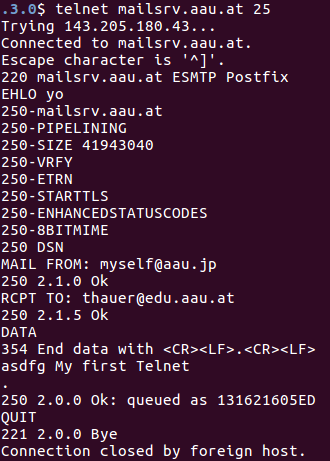
\includegraphics[height=\pagetotal]{TelnetSample.png}

    Alternativ:
    \begin{verbatim}
        telnet -z ssl smtp.gmail.com 465
        HELO
        AUTH LOGIN
        Enter mail-adress in Base64
        Enter Password in Base64
        if Accepted:
        MAIL TO: <mail.com>
        MAIL FROM: <mail.com>
        DATA
        Subect: xy
        asdasd
        .
        QUIT
    \end{verbatim}

    \item Beschreiben Sie das DNS-Protokoll.\\
        Das Domain Name System-Protokoll beschreibt alles rund um das Mapping von IP-Adressen auf Domännamen.
        Man vergibt oft Aliase für zusätzliche Hostnamen, um mit mehreren URLs auf dieselbe IP zugreifen zu können.
        Via Load Distribution kann man intelligentes Hosting ermöglichen, so ist es beispielsweise einen Alias auf eine neue IP ziegen zu lassen.
        VGL.: Hosting von Streaming-Material innerhalb der Server einer anderen Firma.\\

        Bei einem globalen Ausfall vom DNS gilt es die IP-Adressen einzugeben.
        Bei Ausfall eines einzelnen DNS-Servers gibt es keine Einschränkungen aufgrund der Vernetzung der ISPs.
        Prinzipiell hat jeder public Server zumindest 2 Hosts.\\

        Das DNS-Protokoll sieht vor, dass bei der Abfrage eines Server immer der nächstgelegenste ISP kontaktiert wird.
        Je nach Iterativer oder Rekursiver Implementierung geschieht folgendes:
        \begin{addmargin}[1em]{1em}
            \begin{enumerate}[$\diamond$]
                \item Iterativ: Das Usergerät spricht den nächstgelegenen ISP an, welcher mögliche Kontaktdaten des spezifizierten Ziels zurücksendet.
                Dieser fragt anschließend den zurückgegebenen Kontakt ab, bis der richtige Server gefunden wurde und eine Übertragung erfolgen kann.

                \item Rekursiv: Das Usergerät spricht den ISP an, welcher anschließend einen übergeordneten Server abfragt. Sobald der Zielserver gefunden wurde,
                reisen die Kontaktdaten über denselben Weg wieder zurück.

            \end{enumerate}
        \end{addmargin}
\end{enumerate}

\end{document}


%%% Sources:
% https://www.w3.org/Protocols/HTTP/AsImplemented.html
% WebTech-VO-Unterlagen, 2nd.pdf
% RN-chapter-3.pdf
% https://www.thomas-krenn.com/de/wiki/TCP_Port_80_(http)_Zugriff_mit_telnet_%C3%BCberpr%C3%BCfen
% https://tools.ietf.org/html/rfc1945
% https://stackoverflow.com/questions/246859/http-1-0-vs-1-1
% https://linuxmeerkat.wordpress.com/2013/10/10/emailing-from-a-gmail-acount-via-telnet/